\vspace{10pt}

{\centering\subsection*{吴才俊:我学会了骑自行车}}

\addcontentsline{toc}{subsection}{吴才俊:我学会了骑自行车}

\renewcommand{\leftmark}{吴才俊:我学会了骑自行车}

\begin{figure}[htbp]

\centering

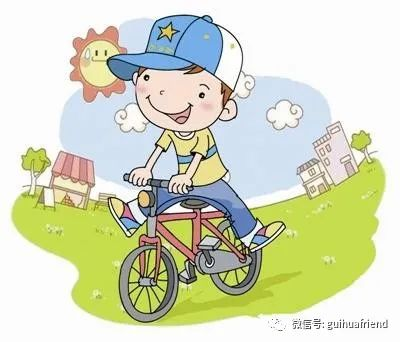
\includegraphics[width = .5\textwidth]{./ch/15.jpg}

\end{figure}



我学会了骑自行车,我很喜欢骑自行车,你们也一定骑过自行车吧?肯定会有人问我为什么要学自行车,因为我看到别人骑自行车,所以就想学了。

我刚开始要有人扶着车,我才敢向前移动,但是别人一松手,我的自行车就会因为重心不稳而倒下。所以我要先从平衡力开始练起,我先找了一块木板,再把木板放在高度平等的水泥块上,再把木板的另一头放在水泥块上,我在上面慢慢地练习。走下来的时候,我发现走独木桥时可以不用双手展开,这样可能会使重心倾斜。所以把两只手保持贴在身上,才会让重心保持在中心。我练习完后再去骑自行车,发现我可以让自行车保持不倒了。

后来我又学会了很多动作,比如单手骑、无手骑、站立骑、不蹬踏板骑和花式动作骑。

我学会了骑自行车,我很开心,这次骑自行车让我知道了什么事情都要努力,不能放弃才能成功。





\vspace{10pt}



作者:四(1)班 吴才俊



指导老师:周瑞



投稿:2021年5月26日



发表:2021年5月27日






                



\vspace{10pt}

\hline



